\section{Offline Selection}\label{sec::selection}

The offline selection focuses on selecting intermediate states \Ds and \KS and resonance states \Dss and \Kstarm. Tables and summarize all selection requirements, which are described in the following paragraph.  Tables 3.1 and 3.2 summarize all selection requirements. The high number of proton-proton interactions during data talking resulted in a large fraction of events having more than one reconstructed PV. These events are called multiple events. There are no multiply events after all selection stages in this analysis, and we didn't perform the best candidates selection. More information can be found in section \ref{subsec::multi}. The preliminary selection of candidates is divided into a selection of each type of particle in the full decay chain. 

\subsection{Selection of \KS}

In LHCb \KS  mesons can be reconstructed using a different type of tracks. The type of track depends on detectors, which particle pass afters proton-proton collision in LHC. Long tracks are reconstructed from hits recorded in VELO, TT detector, and T stations. Downstream are a track of particle which did not pass VELO detector and are reconstructed only from TT and T stations hits. As a result, this particle's mass resolution is worse than for the long track, but the number of candidates is significantly bigger. The number and quality of candidates imply separate selection for long (LL) tracks and downstream (DD).

\begin{table}[h!]
\begin{center}
\begin{tabular}{ p{1cm}p{2cm}p{4.5cm}p{6cm} }
\hline
\hline
  & Variable  & Cut & Justification \\
 \hline
 DD   & $m(\pi\pi)$  & = $m_{\KS(PDG)} \pm$ 20 MeV & Selection genuine \KS\\ 
      & \KS $FD_{sig}$    & $> 7$ & Removing random combinations \\ 
 LL   & $m(\pi\pi)$  & = $m_{\KS(PDG)} \pm$ 20 MeV & Selection genuine \KS\\
 \hline
\end{tabular}
\caption{Offline selection requirements for \KS candidates.}
\label{tab:KS_sel}
\end{center}
\end{table}%

The $FD_{sig}$ stands for fight distance significance defind as:

\begin{equation}
    FD_{sig} = \frac{z_\KS - z_B}{\sqrt{\sigma^2_\KS-\sigma^2_B}}
\end{equation}

where $\sigma_\KS$ and $\sigma_B$  are the errors in the z position of the \KS and \B decay vertex. Flight distance significance is defined as the $z$ distance between the particle and \Bs end vertices divided by the sum in the quadrature of this position's uncertainties. The same requirement is also made for \Ds mesons to separate prompt \Ds mesons created in proton-proton collisions from that one from \B mesons decays. 

The efficiency of selection criteria is calculated using simulated events. Table \ref{tab:KS_eff} show efficiency of each selection requirement for \KS candidates.

\begin{table}[h!]
\begin{center}
\begin{tabular}{ p{1cm}p{2cm}p{4.5cm}p{6cm} }
\hline
\hline
  & Variable  & Cut & Signal Efficiency (\%) \\
 \hline
 DD   & $m(\pi\pi)$  & = $m_{\KS(PDG)} \pm $ 20 MeV & 96.6 \\ 
      & \KS $FD_{sig}$    & $> 7$ & 92.7 \\ 
 LL   & $m(\pi\pi)$  & = $m_{\KS(PDG)} \pm$ 20 MeV & 96.3 \\

 \hline
\end{tabular}
\caption{Efficiency of cuts  (\KS candidates).}
\label{tab:KS_eff}
\end{center}
\end{table}%

\subsection{Selection of \Ds}

The \Ds meson can be reconstructed using 3 decay modes: \Ds\to\Kp\Km\pip, \Ds\to\Kp\pim\pip and \Ds\to\pip\pim\pip since the branching fraction for \Ds\to\Kp\Km\pip is around 5 - 10 times bigger than for \Kp\pim\pip and \pip\pim\pip combination respectively only \Kp\Km\pip combination is considered in this analysis.

\begin{table}[h!]
\centering
\begin{tabular}{ p{4cm}p{4cm} }
\hline
\hline
  Mode & BR \\
 \hline
     \Ds\to\Kp\Km\pip    & (5.45 $\pm$ 0.17) \%  \\
     \Ds\to\Kp\pim\pip    & (0.66 $\pm$ 0.04) \%   \\
     \Ds\to\pip\pim\pip    & (1.09 $\pm$ 0.05) \%   \\
 \hline
\end{tabular}
\caption{Branching fraction of \Ds meson decay to 3$h$ final states}
\label{tab:Ds_br}
\end{table}%

Following requirements was made to remove the combinatorial background from misidentifying of kaons or pions and physical background from misidentification of \Dp or \Lc meson or a random combination of \kaon or \pion with \Dz. This combination can mimic signal final state.

\begin{enumerate}
   \item \Dp\to\Kp\pip\pim \\ 
   Misidentification of kaon from \Ds\to\Kp\Km\pip with \Dp\to\Kp\pim\pip. Removed if the mass of combination under \pion hypothesis is within \Dp $\pm$ 20 MeV mass window unless the combination under \kaon hypothesis is within \Ds $\pm$ 20 MeV mass window and kaon fulfill the stronger requirement of PIDK(\kaon).
   
   \item \Dz\to\Kp\pim or \Dz\to\Kp\Km \\ 
    Combination of \Dz\to\Kp\Km or \Dz\to\Kp\Km meson with random \Kp or \pip. removed if a combination of \Kp\pim or \Kp\Km  $>$ 1850. 
    
   \item \Lc\to\Kp\proton\pim \\ 
   Misidentification of kaon from \Ds\to\Kp\Km\pip with \Lc\to\Kp\proton\pip. Removed if the mass of combination under \proton hypothesis is within \Lc $\pm$ 20 MeV window unless the combination under \kaon hypothesis is within \Ds $\pm$ 20 MeV mass window and kaon fulfill the stronger requirement of PIDK(\kaon).
 \end{enumerate}
 
 
\begin{figure}[h!]
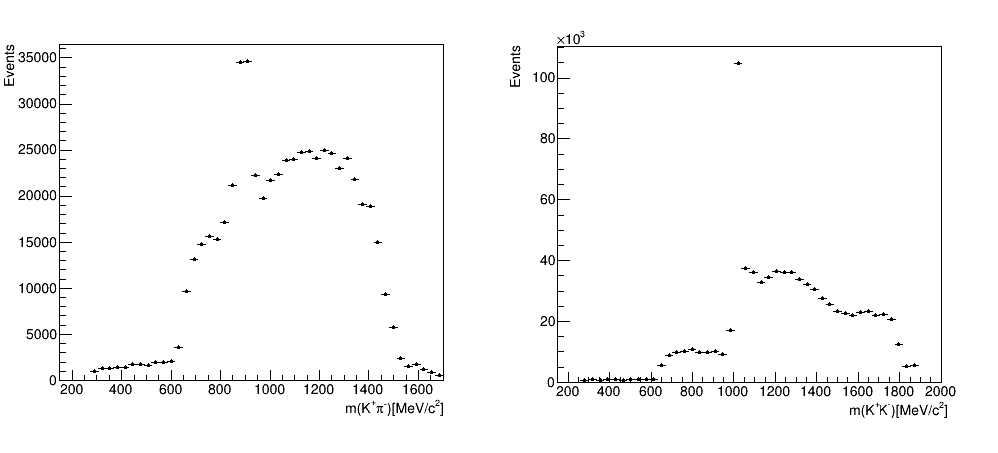
\includegraphics[width=14cm]{figs/Selection/reso.png}
\centering
\caption{Mass distribution of \Kp\Km (left) and \Kp\pim (right) candidates from \Ds\to\Kp\Km\pim (the 2015 data sample).}
\label{fig:reso}
\end{figure}

The Fig. \ref{fig:reso} show contributions from \Lc decay where the \proton is misidentified as \kaon , contributions from \Dz decay where the \pion is misidentified as \kaon, \kaon\pion and \kaon\kaon mass distribution with visible background contribution of \Dz meson. All of them were removed by applying vetos. Histograms were created using the 2015 data sample. 

 Since the \Ds meson decay to the combination of kaons and pions, it can decay by intermediate state \Ds\to(\Pphi\to\Kp\Km)\pip,  \Ds\to \Kp(\Kstarz\to\Km\pip) or by no-resonance mode to \Kp\pim\pip final state. \Pphi and \Kstarz has been investigated, but no additional requirements were made (Fig. \ref{fig:reso}). 

\begin{figure}[h!]
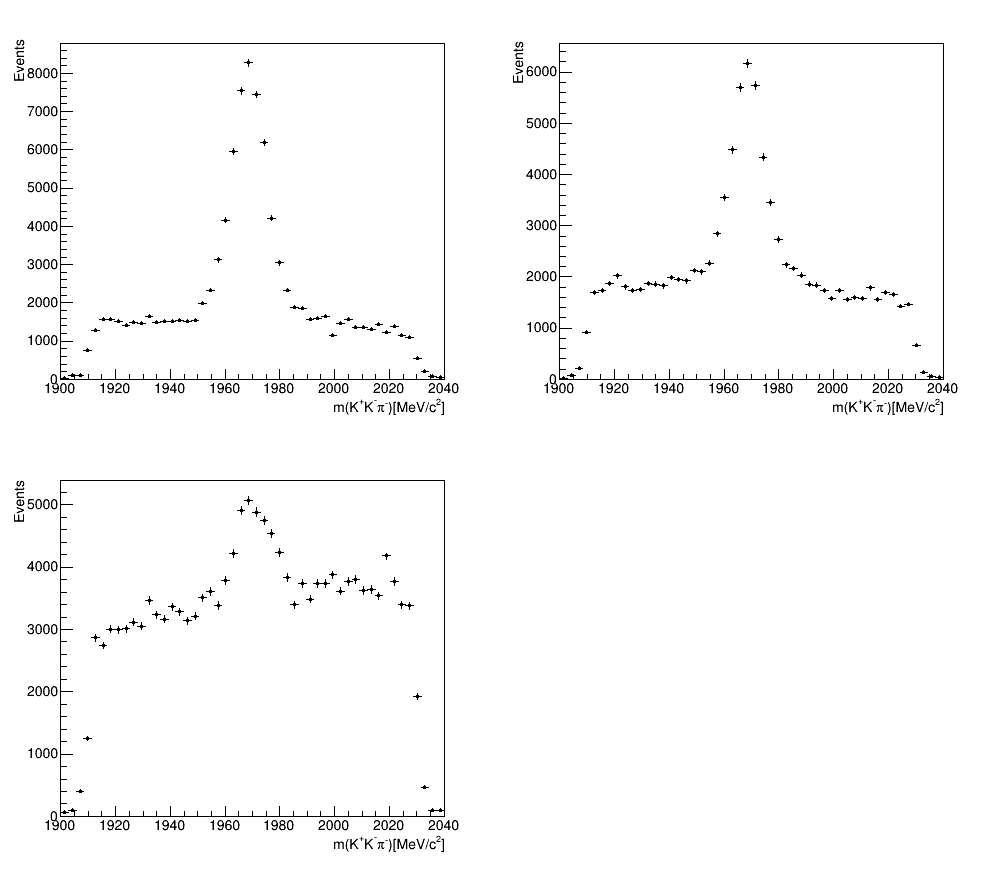
\includegraphics[width=14cm]{figs/Selection/D_reso.png}
\centering
\caption{Mass distribution \Ds\to(\Pphi\to\Kp\Km)\pip (left), \Ds\to \Kp(\Kstarz\to\Km\pip) (right) and no-resonance \Kp\pim\pip candidates mass distribution (bottom, the 2015 data sample).}
\label{fig:D_reso}
\end{figure}
 
The Fig. \ref{fig:D_reso} show \Ds\to(\Pphi\to\Kp\Km)\pip (left), \Ds\to \Kp(\Kstarz\to\Km\pip) (right) and no-resonance \Kp\pim\pip (bottom) candidates mass distribution. Visible is difference between signal to background ratio for each distribution. 

\begin{figure}[h]
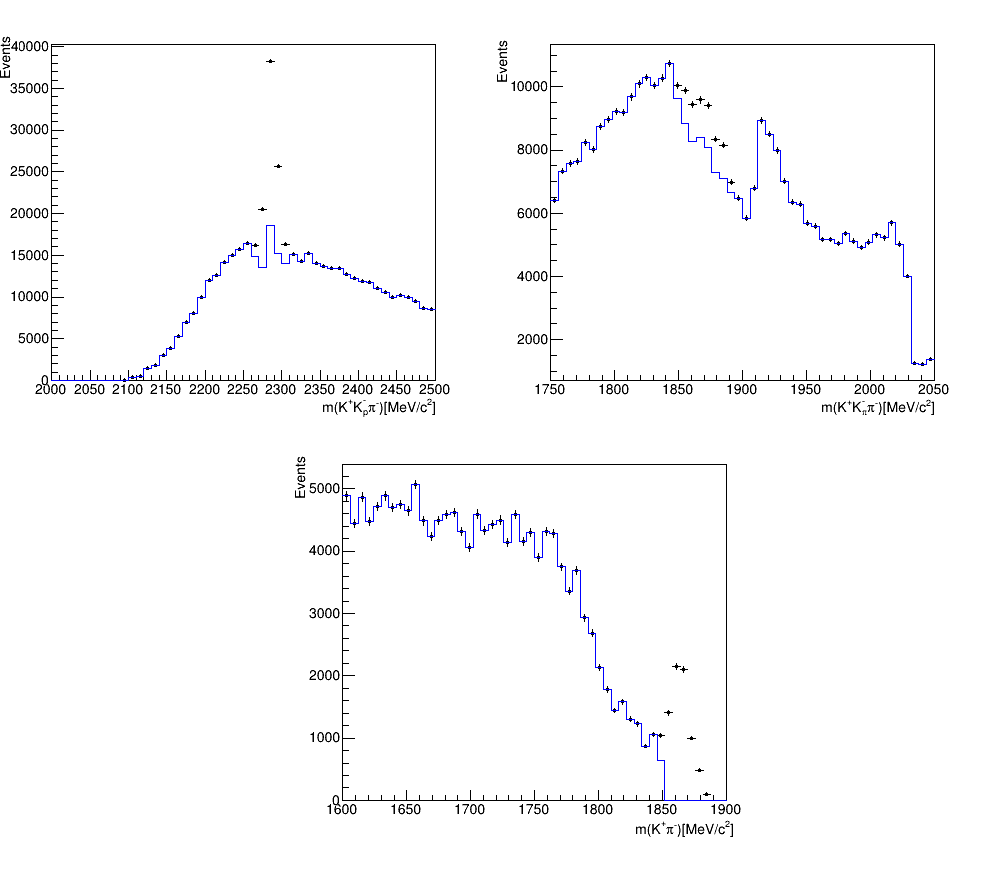
\includegraphics[width=14cm]{figs/Selection/Ds_vetos.png}
\centering
\caption{Background contributions from \Lc decay where the \proton is misidentified as \kaon The \Ds invariant mass is recalculated under proton mass hypothesis for the kaon, black dots are the mass distribution of \Kp\proton\pip before removing \Lc contribution, blue line - after (top left). Background contributions from \Dz decay where the \pion is misidentified as \kaon The \Ds invariant mass is recalculated under pion mass hypothesis for the kaon, black dots are the mass distribution of \Kp\pim\pip before removing \Dz contribution, blue line - after (top right). \kaon\pion and \kaon\kaon mass distribution with visible background contributions from \Dz meson before (black dots) and after (blue line) removing \Dz meson contribution (bottom).}
\label{fig:reso}
\end{figure}
 
 Since the \Dp meson contribution is removed by stripping, we do not expect \Dp mass peak to be visible on $\Kp\Km_{\pim}\pip$ mass distribution. 

\begin{figure}[h!]
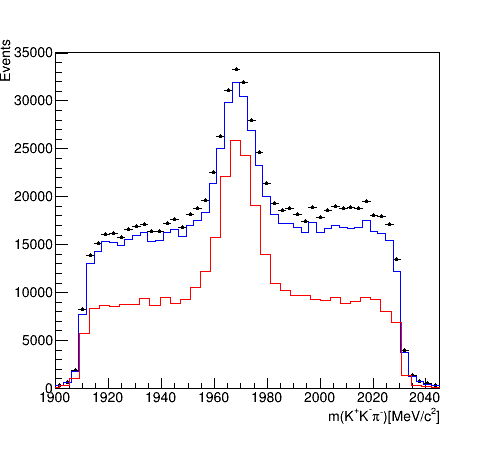
\includegraphics[width=10cm]{figs/Selection/D_mass.png}
\centering
\caption{The \Kp\Km\pip candidates mass distribution after stripping and PID cut (black dot), after applying vetos (blue line), after stripping, PID cut, applying vetos and kinematic cuts (red line, the 2015 data sample). }

\label{fig:D_mass}
\end{figure}

\begin{table}[h!]
\centering
\begin{tabular}{ p{3cm}p{3cm}p{9.5cm}}
\hline
\hline
& Description  & Requirement  \\
\hline
 \Ds\to\Kp\Km\pip   & $m(\Kp\Km\pip)$ & = $m_{\Ds}\pm$ 25 MeV \\ 
                    & PIDK(\kaon)     &   $>$ 5 \\
                    & PIDK(\pion)     &   $<$ 5 \\
                    & hasRich(\kaon / \pion) &    =  1 \\
                    & isMuon(\kaon / \pion) &     =  0 \\
                    & $FD_{sig}$ &     $>$ 0 \\
 & & \\
 \Dz veto   & $m(\Kp\Km)$  & $<$ 1850 MeV \\ 
            & $m(\Kp\pim)$ & $<$ 1850 MeV \\ 
 \Lc veto   & $m(\Kp\Km_{p}\pip)$  & $\neq m(\Lc) \pm 40 $ MeV $||$ PIDK(\Km) - PIDp(\Km) $>$ 5\\ 
 \Dp veto   & $m(\Kp\Km_{\pim}\pip)$  & $\neq m(\Dp) \pm 20 $ MeV $||$ PIDK(\Km) $>$ 7\\ 
 \hline
 \Ds\to\Kp\pim\pip   & $m(\Kp\pim\pip)$ & = $m_{\Ds}\pm$ 25 MeV \\ 
                    & PIDK(\kaon)     &   $>$ 5 \\
                    & PIDK(\pion)     &   $<$ 5 \\
                    & hasRich(\kaon / \pion) &    =  1 \\
                    & isMuon(\kaon / \pion) &     =  0 \\
                    & $FD_{sig}$ &     $>$ 0 \\
 & & \\
 \Dz veto   & $m(\Kp\pim)$ & $<$ 1850 MeV \\ 
 \hline
 \Ds\to\pip\pim\pip & $m(\pip\pim\pip)$ & = $m_{\Ds}\pm$ 25 MeV \\ 
                    & PIDK(\pion)     &   $<$ 0 \\
                    & hasRich(\kaon / \pion) &    =  1 \\
                    & isMuon(\kaon / \pion) &     =  0 \\
                    & $FD_{sig}$ &     $>$ 0 \\
\end{tabular}
\caption{Offline selection requirements for \Ds candidates.}
\label{tab:Ds_sel}
\end{table}%

The efficiency of selection criteria was calculated for kinematic cut of \Ds candidates (Tab. \ref{tab:Ds_eff}).
 
\begin{table}[h!]
\centering
\begin{tabular}{p{3cm}p{4.5cm}p{6cm} }
\hline
\hline
 Variable  & Cut & Signal Efficiency (\%) \\
 \hline
  $m(\Kp\Km\pip)$  & = $m_{\Ds}\pm$ 25 MeV & 83.9 \\ 
  hasRich(\kaon / \pion)    &  =  1 & 99.1 \\ 
  isMuon(\kaon / \pion)  & =  0 & 96.3 \\
  \Ds $FD_{sig}$    &  $>$ 0 & 92.7  \\
 \hline
\end{tabular}
\caption{Efficiency of cuts (\Ds candidates).}
\label{tab:Ds_eff}
\end{table}%

\subsection{Selection of  and \Dss}

Following paragraph describe the selection of resonance states \Dss. The offline selection of  \Dss base on the selection of \Ds mesons and \g.  The selection of \g is done by BDT described in the following paragraph. For \Dss resonances, an additional requirement is made. The $\Delta_M$ variable describes the mass difference between \Dss and \Ds. The mass of the particle is well-known, and the difference of these masses should be around 144 MeV so, $\Delta_M$ requirement is $\Delta_M \in (104,184) $ MeV. 

\begin{table}[h!]
\begin{center}
\begin{tabular}{ p{3cm}p{3cm}p{5.5cm}}
\hline
\hline
& Description  & Requirement  \\
\hline
\Dss  & $\Delta_M $ & $\in (104,184)$ \\ 
\hline

\end{tabular}
\caption{Offline selection requirements for \Dss candidates.}
\label{tab:Reso_sel}
\end{center}
\end{table}%

 
\begin{table}[h!]
\centering
\begin{tabular}{p{3cm}p{4.5cm}p{6cm} }
\hline
\hline
 Variable  & Cut & Signal Efficiency (\%) \\
 \hline
  $\Delta_M $    & $\in (104,184)$  & 82.6 \\ 
 \hline
\end{tabular}
\caption{Efficiency of cuts (\Dss candidates).}
\label{tab:Reso_eff}
\end{table}%


